\documentclass[M3_Night2_Solutions]{subfiles}

\IfSubStr{\jobname}{\detokenize{Solutions}}{\toggletrue{solutions}}{\togglefalse{solutions}}

\fancypagestyle{firstpage}

{\rhead{Night 2 \linebreak \textit{Version: \today}}}

\title{Night 2: Angular Velocity, NEATOs, and Partial Derivatives}
\author{Quantitative Engineering Analysis}
\date{Spring 2019}

\begin{document}

\maketitle
\thispagestyle{firstpage}

\section{Learning Goals}
By the end of this assignment, you should feel confident with the following:
\bi
\item Finding angular velocity from a parametric curve.
\item Interpreting and writing basic programs for the NEATO.
\item Partial Derivatives, and the Chain Rule.
\ei

\section{Angular Velocity Revisited [3 hours]}
Suppose we have a 2D parametric curve $\r(t) = f(t) \ihat + g(t) \jhat$. We saw in the Night 1 assignment that the linear velocity vector is given by $\r'(t) = f'(t) \ihat + g'(t) \jhat$.  

%\begin{marginfigure}
%\begin{center}
%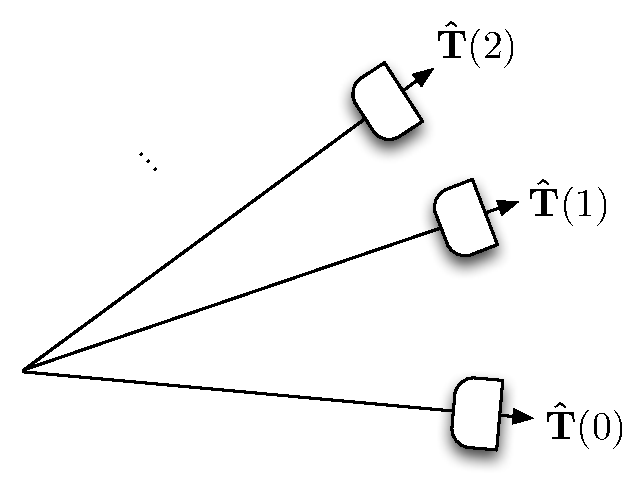
\includegraphics[width=\linewidth]{figures/angular_velocity_derivation}
%\end{center}
%\caption{The change in the robot's heading over time.  The shapes at the end of the arrows are supposed to depict the robot (with the flat side being straightahead).  Since $\hat{\mathbf{T}}$ is a unit vector the robot will move about the unit circle.\label{fig:angularvel}}
%\end{marginfigure}

Determining the expression for the angular velocity $\omega(t)$ of our robot is more involved.  Before we derive the correct expression, we will introduce the notion of angular velocity vectors.  While expressing angular velocity as a vector may at first seem overly complex (since in this case we know that the robot will rotate about the z-axis, and it seems like we should just be able to compute the scalar magnitude along with whether to turn clockwise or counterclockwise), thinking about the angular velocity as a vector will enable our derivation to be done in a much more straightforward and generalizable manner.

Angular velocity vectors point in the direction about which the body rotates (which for our robot will be along either the positive or negative z-axis).  For right-handed coordinate systems (such as the one we are using here), by convention, a positive rotation happens counterclockwise about the direction of the rotation axis.  Further, the magnitude of the angular velocity vector indicates the angular speed.

In the problem at the beginning of class on Monday we discussed the coordinate system attached to the robot:  the body fixed frame.  Because the heading of the robot is locked to the tangent vector $\That$ of the curve, we can think of the vector $\That$ as being a constant in the body fixed frame of the robot.  The body fixed frame is rotating with some unknown angular velocity vector $\boldsymbol \omega$ with respect to the room coordinate system.  If we wish to know the time derivative of the tangent vector $\That=$ in the room coordinate system, we can use the generalized relationship between the time derivatives of vectors in two coordinate systems which are rotating with an angular velocity vector $\boldsymbol \omega$ with respect to each other.  This expression is
\begin{equation}
\frac{d\That}{dt}|_{room} = \frac{d\That}{dt}|_{body} + \boldsymbol \omega \times \That
\end{equation}

(Full mathematical derivation \href{http://envsci.rutgers.edu/~broccoli/dynamics_lectures/lect_06_dyn12_mom_eq_rot.pdf}{here}; nice heuristic explanation \href{https://ocw.mit.edu/courses/aeronautics-and-astronautics/16-07-dynamics-fall-2009/lecture-notes/MIT16_07F09_Lec08.pdf}{here}.) In the body frame of the robot, $\hat{\mathbf{T}}$ is unchanging, since it is always aligned with the forward direction, so the term $\frac{d\hat{\mathbf{T}}}{dt}|_{body}$ is zero leaving us with
\begin{equation}
\frac{d\That}{dt}|_{room} = \boldsymbol \omega \times \That
\end{equation}

%To compute the angular velocity vector we can start from the relationship between rotational and angular velocities.
%\begin{align}
%\mathbf{v}(t) &= \mathbf{\omega}(t) \times \mathbf{r}(t) \nonumber
%\end{align}

%If we substitute in $\hat{\mathbf{T}}(t)$ for $\mathbf{r}(t)$ and

Then we make use of the \href{https://en.wikipedia.org/wiki/Triple_product}{scalar triple product}, which states that $\mathbf{a}\times (\mathbf{b}\times \mathbf{c}) = \mathbf{b}(\mathbf{a}\cdot\mathbf{c}) - \mathbf{c}(\mathbf{a}\cdot\mathbf{b}$).  Using this we can derive our angular velocity vector as follows

%Note: that $\mathbf{v(t)}$ in this case is the derivative of $\hat{\mathbf{T}}(t)$ which is $\mathbf{N}(t)$.

%Note from Emily's revision: I still think the non-unit normal vector is unnecessarily confusing and it seems to be fairly unconventional (i.e., if the students look up the normal vector, they will find info about the *unit* normal). I think it's better to keep it as T-hat-prime. John and I discussed this and he removed N from the previous assignments.
%\begin{align}
%\frac{d\hat{\mathbf{T}}(t)}{dt}|_{lab} &= \textbf{$\Omega$}(t) \times \mathbf{\hat{T}}(t) \nonumber \\
%\mathbf{N}(t) &= \textbf{$\Omega$}(t) \times \mathbf{\hat{T}}(t) \nonumber \\
%\mathbf{\hat{T}}(t) \times \mathbf{N}(t) &= \mathbf{\hat{T}}(t) \times \textbf{$\Omega$}(t) \times \mathbf{\hat{T}}(t) \nonumber \\
%&= \textbf{$\Omega$}(t) (\hat{\mathbf{T}}(t) \cdot \hat{\mathbf{T}}(t) ) - \hat{\mathbf{T}}(t) (\hat{\mathbf{T}}(t) \cdot \textbf{$\Omega$}(t)) \nonumber \\
%&= \textbf{$\Omega$}(t) (1) - \hat{\mathbf{T}}(t) (0) \nonumber \\
%&=  \textbf{$\Omega$}(t) \nonumber \\
%\textbf{$\Omega$}(t) &= \mathbf{\hat{T}}(t) \times \mathbf{N}(t)
%\end{align}


\begin{align}
\frac{d\That}{dt}|_{room} &= \boldsymbol \omega \times \That \nonumber \\
\mathbf{\hat{T}} \times \frac{d\hat{\mathbf{T}}}{dt}|_{room} &= \mathbf{\hat{T}} \times \boldsymbol \omega \times \mathbf{\hat{T}} \nonumber \\
&= \boldsymbol \omega (\hat{\mathbf{T}} \cdot \hat{\mathbf{T}} ) - \hat{\mathbf{T}} (\hat{\mathbf{T}} \cdot \boldsymbol \omega) \nonumber \\
&= \boldsymbol \omega (1) - \hat{\mathbf{T}} (0) \nonumber \\
&=  \boldsymbol \omega \nonumber \\
\Rightarrow \boldsymbol \omega &= \mathbf{\hat{T}} \times \frac{d\hat{\mathbf{T}}}{dt}|_{room}
\end{align}
The x and y components of the angular velocity vector will always be zero because $\hat{\mathbf{T}}$ and $\frac{d\hat{\mathbf{T}}}{dt}|_{room}$ are in the x-y plane and orthogonal.  The magnitude of the z-component is the angular speed.  If the z-component is positive, we turn counterclockwise at that speed.  When it is negative, we  turn clockwise at that speed.

% in the first problem block, make sure to use the series option for enumerate
\begin{enumerate}[series=exercises, label=\textbf{Exercise} (\arabic*)]
\item In the Night 1 assignment you found the unit tangent and normal vectors for various paramaterized curves. We will use that information to find linear and angular velocities, then translate those to left and right wheel velocities for the NEATO.

The vector for a circle is given by: \[ \r(t) = R \cos \alpha t \; \ihat + R \sin \alpha t \; \jhat, \; \alpha t \in [0,2 \pi] \]


Mathematica hints:
\begin{itemize}
\item You can use the apostrophe to take a derivative
\item Specify that $t$ and $\alpha$ are real
\item Include assumptions about coefficients being positive (however, {\bf note that $\alpha$ does not have to be positive})
\item Use the square root of the dot product rather than {\tt Norm}, especially if you're getting a bunch of absolute values in your answer
\item use {\tt Simplify}
\end{itemize}

\begin{enumerate} 
\item What are the linear velocity vector and linear speed?
\solution{ The linear velocity vector is given by $ \v(t) = \r'(t) = x'(t) \ihat + y'(t) \jhat + z'(t) \khat $ or  $\v(t) = v(t) \That(t) $. For the case of the circle, we know: \[\r'(t) = -R\alpha \sin \alpha t \; \ihat + R \alpha \cos \alpha t \; \jhat \]
%and  \begin{eqnarray*}
%\That &=& \frac{\r'}{|\r'|}  \\
%&=& - \sin \alpha t \; \ihat + \cos \alpha t \; \jhat
%\end{eqnarray*}

So, the linear velocity vector is $\v(t) = \alpha R ( - \sin \alpha t \; \ihat + \cos \alpha t \; \jhat)$ and the magnitude (linear speed) is $v(t)= |\alpha| R$ in unts of $\frac{\rm m}{\rm s}$.}

\item What is the unit tangent vector for the circle?
\solution{The unit tangent vector is:
\begin{eqnarray*}
\That &=& \frac{\r'}{|\r'|}  \\
&=& - \sin \alpha t \; \ihat + \cos \alpha t \; \jhat
\end{eqnarray*}
Note that this is independent of $R$ or $\alpha$.}



\item What is the unit normal vector?
\solution{The unit normal vector is
\begin{eqnarray*}
\Nhat &=&   \frac{\That'}{|\That'|} \\
&=& - \cos \alpha t \; \ihat -  \sin \alpha t \; \jhat
\end{eqnarray*}}

\item What is the angular velocity vector?
\solution{ The angular velocity is constant: $\omega=\alpha \khat$.}

\item For the uniform circular motion we have been investigating so far, what does the parameter we have labeled $\alpha$ represent? How is it related to the time it takes to complete one traverse of the circular trajectory?

\solution{The parameter $\alpha$ is the angular frequency of motion, often denoted by $\omega$. For a uniform circular motion, the frequency and angular velocity are equal. The time to complete one traverse ofthe circle is given by the period $T=\frac{2\pi}{\omega}$.}

\item How would you modify this equation for a circle of radius 1 m?
\solution{$R$=1 m}

\item What value would you choose for $\alpha$ if you want your robot to complete the circle in 30 seconds?
\solution{ We know that the product $\alpha t$ must go from $0$ to $2\pi$ for the robot to complete one cycle of the parameterized curve. So, after one complete trip around the circle, $\alpha T = 2 \pi$, so $\alpha= \frac{2 \pi}{T}=0.21$}

\item What are the equations for the left and right wheel velocities for the uniform circle? ($d$=wheel displacement)

\solution{$V_{L}= R|\alpha| - \frac{d \alpha}{2}$ and $V_{R}= R|\alpha| + \frac{d \alpha}{2}$}


\item What are the left and right wheel velocities needed for a 1 m radius counterclockwise circle to be completed in 30 seconds?

\solution{$V_{L}= R\alpha - \frac{d \alpha}{2}$ and $V_{R}= R\alpha + \frac{d \alpha}{2}$\todo{measure wheelbase and update solution here}}


\end{enumerate}

\item The vector for an ellipse is given by:

\[ \r(t) = a \cos \alpha t \; \ihat + b \sin \alpha t \; \jhat, \; \alpha t \in [0,2 \pi] \]

\begin{enumerate}
\item What is the unit tangent vector for the ellipse?

\item What is the linear velocity vector? How does it differ from the example of the circle?

\item What is the unit normal vector?

\item What is the angular velocity vector? How does it differ from the circle?

\item What are the left and right wheel velocities?

\item Plot the linear velocity vector as a function of time for various combinations of the paramters $a$, $b$, and $\alpha$.

\item  Plot the angular velocity vector as a function of time for various combinations of the paramters $a$, $b$, and $\alpha$.

\item  Plot the left and right wheel velocities as a function of time for various combinations of the paramters $a$, $b$, and $\alpha$.

\end{enumerate}

\end{enumerate}

\section {Fun with NEATOs [3 hours]}

In the previous section we found the left and right wheel velocities needed to drive a particular trajectory. In this section of the assignment, we will be thinking about how to translate the velocity vectors to a Matlab program that will control your NEATO.

The control of your NEATO is built on top of the Robotic Operating System (ROS), so you will be using ROS commands to control the velocity values for your robot. We will start by playing with some very basic commands, similar to what you did in class. 

Consider the program below (You can download the code \href{https://drive.google.com/file/d/1sq7yFwfhzcaJakDrcUYzD9HJHjxzhBs8/view?usp=sharing}{here}):

\begin{figure}
\begin{center}
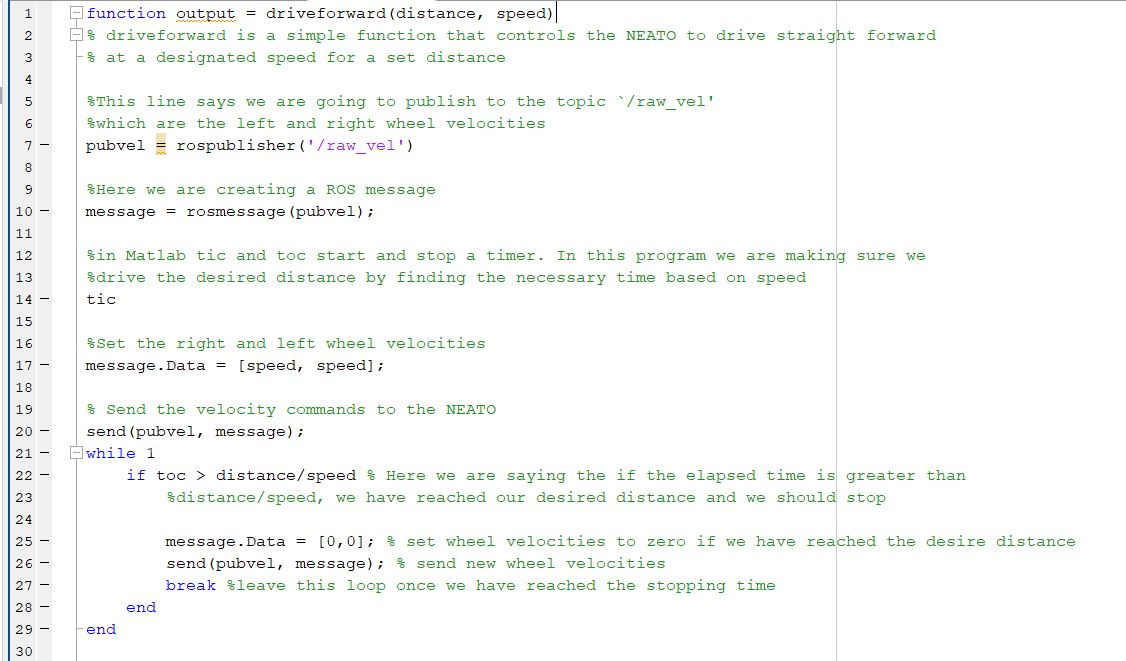
\includegraphics[width=7in]{figs/driveforward.jpg}
\end{center}
\end{figure}

This code snippet defines the function ``driveforward'' which will cause your NEATO to.... you guessed it, drive forward. The function definition is in line 1. You will notice that this function does not have a meaningful output, its sole purpose is to move your robot forward. 

%\begin{enumerate}[resume=exercises, label=\textbf{Exercise} (\arabic*)]
%\item What are the inputs to the function?
%\solution{Inputs are the distance to drive, and at what speed.}
%
%\end{enumerate}

\subsection{The structure of a Simple Robot Program}

Let's break down what is happening in this program:
\begin{itemize}
\item The inputs to the function are the distance to drive, and the speed.
\item Line 7 of the program specifies that you will be publishing to the ROS topic `raw\_vel'. 
\item Line 10 defines a ROS message which will be sent to the `raw\_vel' topic. 
\item In line 14, a timer is started using the ``tic'' command.
\item In line 17, a one by two vector with the left and right wheel velocities is assigned to the Matlab structure ``message.Data''. In this program the velocities are defined at the input to the function, but they could also come from a velocity vector, pre-computed list, etc.
\item In line 20, we use the ``send'' command to send the data in ``message'' to the ROS topic specified by ``pubvel'' (in this case, `raw\_vel')

As soon as we use the ``send'' command, your robot will start moving according to the wheel velocities in `message.Data', and will not stop until we tell it to.  So, what is happening in the rest of this program? At this point, we are not using a distance sensor on the robot. We will introduce those in class on Thursday, but for now we are basing distance off of time and velocity.

\item Line 21 starts a loop that basically monitors how long the robot has been moving forward. 
\item In line 22 we use the ``toc'' command to check how much time has elapsed since ``tic'' was sent. This is very close to the amount of time the robot has been moving. We use the simple fact that $distance=velocity\times time$ to find the elapsed time needed to travel the distance we specified in the function call. We say that if we have reached that maximum time, we send a zero velocity command in lines 25 and 26.
\item If we have not reached the maximum elapsed time for our distance, we stay inside the loop and keep checking the time.

\end{itemize}


%\lstinputlisting{driveforward.m}

%\begin{verbatim}
%
%function output = driveforward(distance, speed);
%% driveforward is a simple function that controls the NEATO to drive straight forward 
%% at a designated speed for a set distance
%
%pubvel = rospublisher('/raw_vel') %This line says we are going to publish to the topic `/raw_vel' 
%%which are the left and right wheel velocities
%
%message = rosmessage(pubvel); %Here we are creating a ROS message
%
%tic %in Matlab tic and toc start and stop a timer. In this program we are making sure we 
%%drive the desired distance by finding the necessary time based on speed
%
%message.Data = [speed, speed]; %Set the right and left wheel velocities 
%
%send(pubvel, message); % Send the velocity commands to the NEATO
%
%while 1
%    if toc > distance/speed % Here we are saying the if the elapsed time is greater than distance/speed, we have reached our desired distance and we should stop
%        
%        message.Data = [0,0]; % set wheel velocities to zero if we have reached the desire distance
%        send(pubvel, message); % send new wheel velocities
%        break %leave this loop once we have reached the stopping time
%    end
%end
%
%end
%
%\end{verbatim}


\begin{enumerate}[resume=exercises, label=\textbf{Exercise} (\arabic*)]
\item Download the above program and open the m-file in Matlab. It is a function, so it can be called from the command window using the form:
\begin{verbatim}
output = driveforward(distance, speed)
\end{verbatim}

Using this new function, try driving the NEATO for several combinations of distances and speeds. Mark the anticipated finish position on the floor with tape or check. Time your robot as it runs. Do the final distance and time match your expectations?
\end{enumerate}

\subsection{Receiving Sensor Data}

In the previous example program we published to a ROS topic to set the NEATO wheel velocities. In ROS you can also subscribe to a topic to do things like receive sensor data. Download and open the program \href{https://drive.google.com/file/d/1DfVy8Nvc7KsOMiJcjBcAhPF8cUOe7-uv/view?usp=sharing}{driveUntilBump} in Matlab.

\begin{enumerate}[resume=exercises, label=\textbf{Exercise} (\arabic*)]

\item In line 2 the `rossubscriber' command is introduced. From the code, what sensor output are we monitoring? 

\item The variable `bumpmessage' is a structure. What is the size of `bumpmessage.data'? What do the values contained in that variable mean?

\item What is the `driveUntilBump' code commanding the robot to do? 
\begin{enumerate}
\item Test the `driveUntilBump' code on a NEATO and verify that your interpretation is correct.
\end {enumerate}

\item Modify the `driveUntilBump' code to make it a function where the robot velocity is an input.

\item Using what you have learned from the examples above, write a program that meets the following requirements:
\begin{enumerate}
\item The program commands the robot to drive a designated distance at a chosen speed, and stops when that distance is reached.
\item If the bump sensor is triggered, the robot reverses direction and backs up for 5 seconds then stops.
\end{enumerate}

Take a short video of your succesful robot, and include the code in your assignment.

Try developing this code on your own first, then if you get stuck, take a look at the program \href{https://drive.google.com/file/d/1whHgaPFppUErc7qB__v0tZ_5z99tzGOz/view?usp=sharing}{driveUntilBumpThenRunAway} for inspiration.

\end{enumerate}


\section{Partial Derivatives and the Chain Rule [2 hours]}

Now work your way through the following sections and problems from the book {\tt Multivariable Calculus by Stewart}, and the book, {\tt A First Course in Mathematical Modeling by Giordano, Fox, and Horton}. You can find pdf copies of the relevant sections on Canvas, subject to the fair use policy. The key material is contained in Section 14.6, although we include a couple of prior sections for completeness.

\begin{enumerate}[resume=exercises, label=\textbf{Exercise} (\arabic*)]
\item Please read Section 14.3 from \href{https://drive.google.com/file/d/1PMW_Smnfv3_aJ85pzC-yCx52dAQNWZNT/view?usp=sharing}{Stewart} on Partial Derivatives. Take notes on important concepts and definitions. 

\item Please read Section 14.5 from \href{https://drive.google.com/file/d/1PMW_Smnfv3_aJ85pzC-yCx52dAQNWZNT/view?usp=sharing}{Stewart} on The Chain Rule. Take notes on important concepts and definitions.

This is new material on extending the notion of the chain rule from functions of one variable to functions of many variables. The main results are captured in the pink boxes labeled 1 through 4 - these are various cases of the chain rule. Again, this text is written for a student who doesn't have linear algebra. As you read these rules, think about how you might use matrix notation to make this cleaner and more compact. At this stage you should ignore the section on Implicit Derivatives - it will be too confusing and take too long. 

Do the following exercises by hand and check your work in Mathematica.

\item Complete question 1 from 14.5 Exercises.
\item Complete question 5 from 14.5 Exercises.
\item Complete question 11 from 14.5 Exercises.

\end{enumerate}



\end{document}
